\section{Additional Monte Carlo results}\label{app:mc}

\begin{table}[t]
\centering
\caption{Monte Carlo results}\label{tab:mc}
\scriptsize
\resizebox{\textwidth}{!}{% Monte Carlo summary for EW-DRPL. Requires \usepackage{booktabs}.
% Cells: mean (MC standard error) over 200 replications.
\begin{tabular}{lcccccc}
\toprule
 & \multicolumn{3}{c}{$N=150$} & \multicolumn{3}{c}{$N=500$} \\
\cmidrule(lr){2-4}\cmidrule(lr){5-7}
Method & $\varepsilon=0$ & $\varepsilon=1$ & $\varepsilon=2$ & $\varepsilon=0$ & $\varepsilon=1$ & $\varepsilon=2$ \\
\midrule
\multicolumn{7}{l}{\emph{Panel A: regret vs.\ oracle tree (true welfare)}} \\
EW-DRPL & 0.058 (0.002) & 0.070 (0.002) & 0.070 (0.005) & 0.028 (0.001) & 0.047 (0.002) & 0.051 (0.003) \\
EW-DRPL-crossfit & 0.057 (0.001) & 0.073 (0.002) & 0.079 (0.005) & 0.032 (0.001) & 0.050 (0.002) & 0.056 (0.003) \\
Utilitarian-DR & 0.058 (0.002) & 0.078 (0.002) & 0.106 (0.008) & 0.028 (0.001) & 0.052 (0.002) & 0.085 (0.007) \\
Plug-in & 0.046 (0.002) & 0.062 (0.002) & 0.069 (0.007) & 0.027 (0.001) & 0.043 (0.002) & 0.048 (0.004) \\
IPW-only & 0.064 (0.001) & 0.076 (0.002) & 0.074 (0.006) & 0.053 (0.001) & 0.075 (0.001) & 0.077 (0.005) \\
Raw-psi-DR & 0.066 (0.001) & 0.078 (0.002) & 0.083 (0.006) & 0.050 (0.001) & 0.069 (0.002) & 0.084 (0.006) \\
Naive-TWFE & 0.078 (0.001) & 0.105 (0.002) & 0.156 (0.009) & 0.077 (0.000) & 0.106 (0.001) & 0.166 (0.008) \\
Oracle & 0.000 (0.000) & 0.000 (0.000) & 0.000 (0.000) & 0.000 (0.000) & 0.000 (0.000) & 0.000 (0.000) \\
\midrule
\multicolumn{7}{l}{\emph{Panel B: share of oracle-treated countries recovered}} \\
EW-DRPL & 0.393 (0.010) & 0.376 (0.011) & 0.355 (0.009) & 0.584 (0.010) & 0.505 (0.013) & 0.419 (0.011) \\
EW-DRPL-crossfit & 0.405 (0.009) & 0.368 (0.009) & 0.355 (0.008) & 0.556 (0.008) & 0.488 (0.010) & 0.408 (0.008) \\
Utilitarian-DR & 0.393 (0.010) & 0.351 (0.010) & 0.336 (0.010) & 0.584 (0.010) & 0.467 (0.010) & 0.454 (0.010) \\
Plug-in & 0.478 (0.012) & 0.422 (0.011) & 0.396 (0.010) & 0.619 (0.012) & 0.532 (0.014) & 0.454 (0.013) \\
IPW-only & 0.363 (0.009) & 0.330 (0.010) & 0.321 (0.008) & 0.420 (0.008) & 0.332 (0.008) & 0.293 (0.008) \\
Raw-psi-DR & 0.349 (0.009) & 0.334 (0.009) & 0.326 (0.009) & 0.435 (0.009) & 0.373 (0.010) & 0.338 (0.009) \\
Naive-TWFE & 0.118 (0.006) & 0.325 (0.005) & 0.327 (0.004) & 0.093 (0.005) & 0.342 (0.003) & 0.338 (0.003) \\
Oracle & 1.000 (0.000) & 1.000 (0.000) & 1.000 (0.000) & 1.000 (0.000) & 1.000 (0.000) & 1.000 (0.000) \\
\midrule
\multicolumn{7}{l}{\emph{Panel C: ATE of $\rho$ (average over countries and deciles): bias (MC SE) and RMSE}} \\
ATE-DR & -0.057 (0.076) & 1.075 &  & 0.010 (0.005) & 0.072 &  \\
ATE-DR-raw & 0.052 (0.034) & 0.477 &  & -0.000 (0.006) & 0.086 &  \\
ATE-plugin & 0.036 (0.023) & 0.330 &  & 0.011 (0.005) & 0.069 &  \\
ATE-IPW & 0.077 (0.037) & 0.526 &  & 0.022 (0.006) & 0.084 &  \\
ATE-naive & 0.291 (0.006) & 0.303 &  & 0.300 (0.003) & 0.303 &  \\
\bottomrule
\end{tabular}
}
\begin{minipage}{\textwidth}\footnotesize\smallskip
\emph{Notes:} 200 replications; Monte Carlo standard errors in parentheses. Regret is the
difference between the welfare of the oracle depth-2 tree and that of the learned rule, both
evaluated with the true benefits under the indicated inequality aversion $\epsilon$. Budget
$k=0.3$. ``crossfit'' learns the tree on four country folds and applies it to the fifth.
Propensity scores are clipped to $[0.1,0.9]$.
\end{minipage}
\end{table}

\begin{table}[htbp]
\centering
\caption{Monte Carlo: propensity trimming and the doubly robust estimator}\label{tab:mc_trim}
\small
\begin{tabular}{lcccccc}
\toprule
 & & \multicolumn{2}{c}{Average effect} & \multicolumn{3}{c}{EW-DRPL regret} \\
\cmidrule(lr){3-4}\cmidrule(lr){5-7}
Trimming & $N$ & Bias & RMSE & $\epsilon=0$ & $\epsilon=1$ & $\epsilon=2$ \\
\midrule
$[0.05,0.95]$ & 150 & -0.057 & 1.075 & 0.058 & 0.070 & 0.070 \\
$[0.05,0.95]$ & 500 & 0.010 & 0.072 & 0.028 & 0.047 & 0.051 \\
$[0.1,0.9]$ & 150 & -0.012 & 0.559 & 0.055 & 0.068 & 0.067 \\
$[0.1,0.9]$ & 500 & 0.011 & 0.065 & 0.027 & 0.044 & 0.048 \\
\bottomrule
\end{tabular}
\begin{minipage}{0.95\textwidth}\footnotesize\smallskip
\emph{Notes:} 200 replications of the design in Section~\ref{sec:mc} under each trimming rule.
\end{minipage}
\end{table}


\section{Additional results for cereal yields}\label{app:agri}

\begin{table}[t]
\centering
\caption{Heat shocks and cereal-yield growth: first stage}\label{tab:firststage}
\small
\begin{tabular}{lcccc}
\toprule
Sample & Coefficient (SE) & $p$ & Observations & Countries \\
\midrule
All countries & $-3.572$ (0.530) & $<0.001$ & 3,679 & 155 \\
EMDEs & $-2.684$ (0.759) & $<0.001$ & 2,538 & 107 \\
Baseline temp.\ $\geq 20^{\circ}$C & $-0.336$ (0.908) & 0.711 & 1,971 & 83 \\
Annual-mean anomaly as regressor & $-0.612$ (1.006) & 0.543 & 3,679 & 155 \\
\bottomrule
\end{tabular}
\begin{minipage}{0.95\textwidth}\footnotesize\smallskip
\emph{Notes:} Dependent variable: $100\times\Delta\ln$ cereal yield (kg/ha). Regressor: hottest-month
mean temperature minus its 1980--2023 country-specific linear trend ($^{\circ}$C), except in the last
row. Country and year fixed effects; standard errors clustered by country. Observations with
$|\Delta\ln\text{yield}|\geq 1$ are dropped as data errors. The sample is larger than the estimation
sample of Table~\ref{tab:ate}, which also requires the lagged covariates.
\end{minipage}
\end{table}

\begin{table}[htbp]
\centering
\caption{Sorted group effects (GATES) and classification analysis (CLAN), cereal yields}\label{tab:gates}
\small
\begin{tabular}{lcccccc}
\toprule
 & Q1 & Q2 & Q3 & Q4 & Q5 & Q5$-$Q1 (SE) \\
\midrule
Mean $\Gamma$ & -1.49 & 2.76 & -0.06 & -3.82 & 3.90 & 5.39 (3.59) \\
 & (3.01) & (2.31) & (2.59) & (2.14) & (1.95) & \\ \midrule
Log GDP per capita & 9.62 & 9.44 & 9.36 & 9.22 & 9.24 & -0.38 (0.22) \\
Gini index & 36.71 & 38.76 & 38.18 & 38.58 & 39.12 & 2.41 (1.15) \\
Internet users (\%) & 48.84 & 42.32 & 36.93 & 29.34 & 29.63 & -19.21 (4.76) \\
Agriculture share (\%) & 10.93 & 10.97 & 11.51 & 12.55 & 12.68 & 1.75 (1.97) \\
Baseline temperature & 17.25 & 17.75 & 17.58 & 17.94 & 17.42 & 0.17 (1.42) \\
Knowledge sovereignty & 0.18 & 0.19 & 0.20 & 0.14 & 0.08 & -0.11 (0.04) \\
\bottomrule
\end{tabular}
\begin{minipage}{0.95\textwidth}\footnotesize\smallskip
\emph{Notes:} Country-years sorted into quintiles of out-of-fold predicted resilience
$\hat m_1-\hat m_0$. First row: mean doubly robust score with country-clustered SE. Remaining rows:
feature means by quintile.
\end{minipage}
\end{table}


\begin{table}[htbp]
\centering
\caption{Average heat damage on the estimation sample under alternative estimators}\label{tab:recon}
\small
\begin{tabular}{lc}
\toprule
Estimator & Damage per $^{\circ}$C (SE) \\
\midrule
Two-way fixed effects (country, year) & $-$3.579 (0.552) \\
Year and region fixed effects, lagged covariates & $-$3.171 (0.531) \\
EW-DRPL mean orthogonal slope score $\psi^*$ & $-$1.517 (0.536) \\
EW-DRPL mean $\psi^*$, median over splits & $-$1.382 \\
\bottomrule
\end{tabular}
\begin{minipage}{0.9\textwidth}\footnotesize\smallskip
\emph{Notes:} 3,336 country-years in 145 countries. Dependent variable: cereal-yield growth (\%);
shock: hottest-month anomaly. Standard errors clustered by country.
\end{minipage}
\end{table}


\begin{table}[htbp]
\centering
\caption{Held-out welfare value of allocation rules, unweighted objective}\label{tab:unweighted}
\small
\begin{tabular}{lcccc}
\toprule
Rule & $\epsilon=0$ & $\epsilon=0.5$ & $\epsilon=1$ & $\epsilon=2$ \\
\midrule
EW-DRPL ($\epsilon$-specific tree) & $-$0.126 & $-$0.326 & $-$0.093 & 0.027 \\
 & {\footnotesize[$-$0.53, 0.26]} & {\footnotesize[$-$1.12, 0.38]} & {\footnotesize[$-$1.18, 0.85]} & {\footnotesize[$-$0.75, 0.91]} \\
Utilitarian tree & $-$0.126 & $-$0.344 & $-$0.584 & $-$0.544 \\
 & {\footnotesize[$-$0.53, 0.26]} & {\footnotesize[$-$1.16, 0.37]} & {\footnotesize[$-$1.91, 0.44]} & {\footnotesize[$-$2.65, 1.33]} \\
Plug-in tree & 0.067 & 0.110 & 0.279 & 1.032 \\
 & {\footnotesize[$-$0.31, 0.44]} & {\footnotesize[$-$0.58, 0.78]} & {\footnotesize[$-$0.79, 1.27]} & {\footnotesize[$-$0.50, 3.02]} \\
Capable-first & $-$0.048 & $-$0.025 & 0.019 & 0.068 \\
 & {\footnotesize[$-$0.13, 0.04]} & {\footnotesize[$-$0.13, 0.11]} & {\footnotesize[$-$0.10, 0.20]} & {\footnotesize[$-$0.05, 0.25]} \\
Poorest-first & $-$0.005 & $-$0.026 & $-$0.025 & 0.343 \\
 & {\footnotesize[$-$0.37, 0.32]} & {\footnotesize[$-$0.83, 0.68]} & {\footnotesize[$-$1.35, 1.16]} & {\footnotesize[$-$1.93, 2.46]} \\
Most-agricultural-first & 0.079 & 0.053 & 0.022 & 0.333 \\
 & {\footnotesize[$-$0.34, 0.43]} & {\footnotesize[$-$0.79, 0.74]} & {\footnotesize[$-$1.33, 1.19]} & {\footnotesize[$-$1.93, 2.45]} \\
Random (expected) & 0.050 & 0.049 & 0.035 & 0.100 \\
 & {\footnotesize[$-$0.09, 0.20]} & {\footnotesize[$-$0.23, 0.29]} & {\footnotesize[$-$0.41, 0.40]} & {\footnotesize[$-$0.55, 0.74]} \\
\bottomrule
\end{tabular}
\begin{minipage}{0.95\textwidth}\footnotesize\smallskip
\emph{Notes:} As Table~\ref{tab:policy}, but each country receives equal weight in the objective and
in the normalisation of the Atkinson weights (no population scaling).
\end{minipage}
\end{table}


\begin{figure}[htbp]
\centering
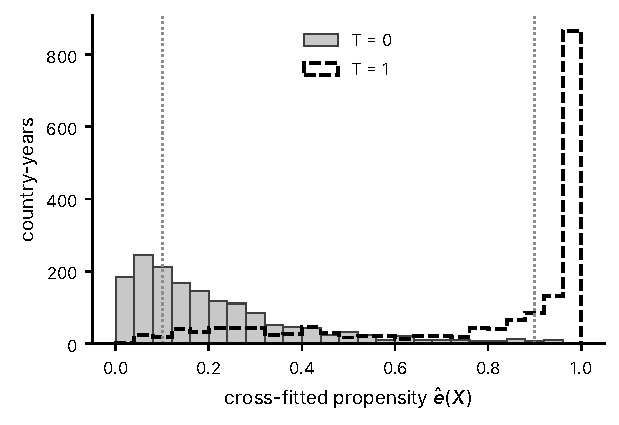
\includegraphics[width=0.75\textwidth]{fig_agri_overlap.pdf}
\caption{Cross-fitted propensity scores for income-adjusted climate-AI capability, by capability
status. Dotted lines mark the trimming bounds 0.1 and 0.9.}
\label{fig:overlap}
\end{figure}

\section{Decile income growth, aggregate growth and costs}\label{app:decile}

This appendix applies EW-DRPL directly to the distributional data. Decile mean income or
consumption comes from the World Bank's Poverty and Inequality Platform. For each country we keep
national surveys of one welfare concept and form spells from consecutive surveys that the
platform flags as comparable and that are at most ten years apart. The outcome is the annualised
log growth of each decile's mean, winsorised at the 1st and 99th percentiles within decile, and
the shock is the mean annual temperature anomaly over the spell. The estimation sample contains
1,334 spells in 124 countries.

Table~\ref{tab:decile} reports the decile-specific resilience effects. The point estimates are more
negative for the poorer deciles, but none is distinguishable from zero, and the average changes sign
across sample splits (from $-4.6$ to $4.1$). The underlying problem is the first stage: the annual
temperature anomaly has no detectable effect on GDP per capita growth in our sample
($-0.10$, SE 0.18; in hot EMDEs $-0.27$, SE 0.46), and spell averages dilute it further. Applied to
country-year GDP growth, the average resilience effect is 0.12 (SE 0.50); in this supplementary
analysis the covariates are measured in the same year as the outcome. Table~\ref{tab:cost}
reports the cost module.

\begin{table}[htbp]
\centering
\caption{Decile income growth: resilience incidence and marginal damages}\label{tab:decile}
\small
\begin{tabular}{lccc}
\toprule
Decile & Resilience effect $E[\Gamma_d]$ & Damage, $T=1$ & Damage, $T=0$ \\
\midrule
1 & -3.11 (2.40) & -0.37 (1.11) & -0.23 (1.13) \\
2 & -2.12 (1.99) & -0.18 (0.73) & 0.27 (0.78) \\
3 & -2.30 (1.92) & -0.23 (0.65) & 0.64 (0.75) \\
4 & -2.04 (1.94) & -0.01 (0.64) & 0.97 (0.68) \\
5 & -1.73 (1.86) & 0.14 (0.59) & 1.12 (0.63) \\
6 & -1.53 (1.85) & 0.21 (0.56) & 1.16 (0.58) \\
7 & -1.39 (1.68) & 0.27 (0.52) & 1.19 (0.57) \\
8 & -0.82 (1.78) & 0.23 (0.53) & 1.07 (0.59) \\
9 & -0.74 (1.74) & -0.00 (0.56) & 1.05 (0.64) \\
10 & 0.02 (1.76) & 0.62 (0.63) & 1.07 (0.82) \\
\midrule Average & -1.58 (1.80) & & \\
\bottomrule
\end{tabular}
\begin{minipage}{0.95\textwidth}\footnotesize\smallskip
\emph{Notes:} 1,334 survey spells in 124 countries (13,340 spell-decile observations). Outcome:
annualised growth of decile mean income or consumption (\%). Shock: mean annual temperature
anomaly over the spell. Capability: income-adjusted climate-AI stock at the start of the spell.
Scores are medians over 20 sample splits; country-clustered SE in parentheses. Damage columns:
mean orthogonal slope score $\psi^*_d$ by capability status.
\end{minipage}
\end{table}


\begin{table}[htbp]
\centering
\caption{The energy and emissions cost of AI capability (double machine learning)}\label{tab:cost}
\small
\resizebox{\textwidth}{!}{%
\begin{tabular}{lcccccc}
\toprule
 & \multicolumn{3}{c}{Log electricity per capita} & \multicolumn{3}{c}{Log CO$_2$ per capita} \\
\cmidrule(lr){2-4}\cmidrule(lr){5-7}
Treatment & Climate-AI stock & AI output & Income residual & Climate-AI stock & AI output & Income residual \\
\midrule
Coefficient (SE) & -0.015 (0.112) & 0.070 (0.060) & -0.046 (0.112) & 0.061 (0.099) & 0.028 (0.056) & 0.054 (0.099) \\
$p$-value & 0.894 & 0.243 & 0.679 & 0.538 & 0.613 & 0.587 \\
High $-$ low renewable share & 0.247 (0.202) & 0.119 (0.098) & 0.423 (0.204) & 0.075 (0.186) & 0.088 (0.108) & 0.196 (0.189) \\
Country-years & 3192 & 3192 & 3192 & 3192 & 3192 & 3192 \\
\bottomrule
\end{tabular}}
\begin{minipage}{0.95\textwidth}\footnotesize\smallskip
\emph{Notes:} Partially linear model with cross-fitted gradient-boosting nuisances (five country
folds) and Mundlak country means of all controls (log GDP per capita, urban share, log population,
internet use, agricultural share, renewable share, baseline temperature, year). 149 countries,
2001--2022. SE clustered by country. Climate-AI stock: $\ln(1+K/\text{pop})$, lagged; AI output:
$\ln(1+$AI works per million$)$, lagged; income residual: capability beyond income (continuous).
\end{minipage}
\end{table}


\section{Additional allocation and solver results}\label{app:allocation}

\begin{table}[htbp]
\centering
\caption{Share of agricultural heat exposure covered at a budget of 37 countries}
\label{tab:coverage}
\small
\begin{tabular}{lrrrr}
\toprule
 & & \multicolumn{3}{c}{Share of sample exposure (\%)}\\
\cmidrule(lr){3-5}
Rule & EMDEs & $\epsilon=0$ & $\epsilon=1$ & $\epsilon=1$\\
 & selected & & Bottom-first & Uniform\\
\midrule
Research-first          &  5 &  3.3 &  1.5 &  0.9 \\
Poorest-first           & 37 & 58.8 & 72.8 & 77.6 \\
Most-agricultural-first & 37 & 63.3 & 78.4 & 83.1 \\
Random (expected)       & 25.3 & 29.4 & 29.4 & 29.4 \\
\bottomrule
\end{tabular}
\begin{minipage}{0.95\textwidth}\footnotesize\smallskip
\emph{Notes.} The sample contains 126 countries, including 86 emerging and developing
economies. The rules rank countries by the country mean of log one
plus lagged climate-AI stock per million people, the country mean of lagged log GDP per capita,
or average agricultural employment share. Columns report
Equation~\eqref{eq:coverage}. At $\epsilon=0$, exposure is proportional to 2023 population
times agricultural employment share times the standard deviation of hottest-month
temperature anomalies. At $\epsilon=1$, the exposure assigned to each income decile
is weighted by the inverse of mean decile income. Bottom-first assigns agricultural
exposure to poorer deciles first; uniform allocates the same exposure fraction to
each decile. The shares use a common slope improvement and can be reproduced with
\texttt{code/31\_application\_agri.py --exposure-shares 0.3}.
\end{minipage}
\end{table}


\begin{table}[htbp]
\centering
\small
\caption{Quota-preserving rules on independent simulated test countries}
\label{tab:swap_simulation}
\begin{tabular}{lrrr}
\toprule
Rule & Gain (MC SE) & Regret & Loss rate (\%) \\
\midrule
\multicolumn{4}{l}{\emph{Moderate overlap}} \\
Exposure baseline & 0.0000 (0.0000) & 0.0373 & 0.0 \\
DR swaps & 0.0055 (0.0012) & 0.0318 & 36.4 \\
Plug-in swaps & 0.0097 (0.0012) & 0.0275 & 30.8 \\
Mean-score swaps & 0.0106 (0.0012) & 0.0266 & 26.8 \\
Robust swaps & 0.0104 (0.0010) & 0.0269 & 27.2 \\
\midrule
\multicolumn{4}{l}{\emph{Weak overlap}} \\
Exposure baseline & 0.0000 (0.0000) & 0.0373 & 0.0 \\
DR swaps & 0.0052 (0.0010) & 0.0320 & 40.6 \\
Plug-in swaps & 0.0078 (0.0011) & 0.0294 & 35.8 \\
Mean-score swaps & 0.0080 (0.0011) & 0.0292 & 36.2 \\
Robust swaps & 0.0096 (0.0009) & 0.0276 & 29.0 \\
\midrule
\multicolumn{4}{l}{\emph{Homogeneous effects}} \\
Exposure baseline & 0.0000 (0.0000) & 0.0000 & 0.0 \\
DR swaps & -0.0219 (0.0009) & 0.0219 & 99.0 \\
Plug-in swaps & -0.0226 (0.0010) & 0.0226 & 97.4 \\
Mean-score swaps & -0.0195 (0.0008) & 0.0195 & 97.8 \\
Robust swaps & -0.0149 (0.0008) & 0.0149 & 87.0 \\
\bottomrule
\end{tabular}

\begin{minipage}{0.9\textwidth}\footnotesize\smallskip
\emph{Notes.} 500 replications per design. Every rule selects 90 of 300 test
countries. Gain is the mean equity-weighted welfare change from the exposure
reference. Regret is relative to the best member of the training-derived library
evaluated with the true test-country benefits. Loss rate is the fraction of
replications with a strictly negative gain, allowing a numerical tolerance.
\end{minipage}
\end{table}

\begin{table}[htbp]
\centering
\small
\caption{Estimated welfare changes relative to exposure-based allocation}
\label{tab:swap_application}
\begin{tabular}{lrr}
\toprule
Rule & Gain [95\% interval] & Replacements \\
\midrule
\multicolumn{3}{l}{\emph{Country folds}} \\
Exposure baseline & 0.000 [0.000, 0.000] & 0 \\
DR swaps & 0.000 [-0.704, 0.750] & 20 \\
Plug-in swaps & -0.069 [-0.558, 0.581] & 19 \\
Mean-score swaps & -0.164 [-0.896, 0.586] & 24 \\
Robust swaps & 0.455 [-0.122, 1.219] & 21 \\
\midrule
\multicolumn{3}{l}{\emph{Region folds}} \\
Exposure baseline & 0.000 [0.000, 0.000] & 0 \\
DR swaps & 0.492 [-0.102, 1.504] & 8 \\
Plug-in swaps & 0.378 [-0.295, 1.405] & 13 \\
Mean-score swaps & 0.451 [-0.224, 1.464] & 7 \\
Robust swaps & 0.065 [-0.184, 0.403] & 14 \\
\bottomrule
\end{tabular}

\begin{minipage}{0.9\textwidth}\footnotesize\smallskip
\emph{Notes.} All rules allocate 37 places across 126 eligible countries. Gain is the
mean difference in equity-weighted welfare using the same orthogonal score with the
propensity clipped at 0.10 for evaluation. Country bootstrap intervals condition on
the learned rules and scores. Replacements count the places allocated to countries
outside the batch-specific reference allocation. The two designs use different
batch definitions and therefore different reference assignments.
\end{minipage}
\end{table}

\begin{table}[htbp]
\centering
\small
\caption{Independent test-country performance of integer portfolios}
\label{tab:ellipsoid_simulation}
\begin{tabular}{lrrr}
\toprule
Rule & Mean gain & Mean regret & Loss rate (\%) \\
\midrule
\multicolumn{4}{l}{\emph{Moderate overlap}} \\
Exposure reference & 0.0000 & 0.0430 & 0.0 \\
Threshold swaps & 0.0109 & 0.0321 & 26.0 \\
Pooled mean & 0.0176 & 0.0254 & 18.5 \\
Ellipsoidal portfolio & 0.0131 & 0.0299 & 5.0 \\
\midrule
\multicolumn{4}{l}{\emph{Weak overlap}} \\
Exposure reference & 0.0000 & 0.0430 & 0.0 \\
Threshold swaps & 0.0076 & 0.0353 & 26.5 \\
Pooled mean & 0.0130 & 0.0300 & 22.5 \\
Ellipsoidal portfolio & 0.0129 & 0.0301 & 3.5 \\
\midrule
\multicolumn{4}{l}{\emph{Homogeneous effects}} \\
Exposure reference & 0.0000 & 0.0000 & 0.0 \\
Threshold swaps & $-0.0130$ & 0.0130 & 80.0 \\
Pooled mean & $-0.0206$ & 0.0206 & 99.0 \\
Ellipsoidal portfolio & $-0.0021$ & 0.0021 & 30.5 \\
\bottomrule
\end{tabular}
\begin{minipage}{0.9\textwidth}\footnotesize\smallskip
\emph{Notes.} 200 replications per design. All rules choose 18 of 60 independent test
countries. Gain uses the true benefits relative to the exposure reference. Regret
uses the unrestricted best portfolio at the same quota. Loss rate is the frequency
of a strictly negative gain. The pooled mean and ellipsoidal portfolios use the
same fitted benefit surface.
\end{minipage}
\end{table}


\begin{table}[htbp]
\centering
\small
\caption{Integer portfolios in held-out agricultural country and region folds}
\label{tab:ellipsoid_application}
\begin{tabular}{lrr}
\toprule
Rule & Gain [95\% interval] & Replacements \\
\midrule
\multicolumn{3}{l}{\emph{Country folds}} \\
Exposure reference & 0.000 [0.000, 0.000] & 0 \\
Threshold swaps & 0.455 [$-0.122$, 1.219] & 21 \\
Pooled mean & 0.054 [$-0.735$, 0.916] & 27 \\
Ellipsoidal portfolio & $-0.271$ [$-0.754$, $-0.009$] & 7 \\
\midrule
\multicolumn{3}{l}{\emph{Region folds}} \\
Exposure reference & 0.000 [0.000, 0.000] & 0 \\
Threshold swaps & 0.065 [$-0.184$, 0.403] & 14 \\
Pooled mean & $-0.048$ [$-1.019$, 1.136] & 25 \\
Ellipsoidal portfolio & 0.000 [0.000, 0.000] & 0 \\
\bottomrule
\end{tabular}
\begin{minipage}{0.9\textwidth}\footnotesize\smallskip
\emph{Notes.} 37 places across 126 countries in each design. Gains use the same
held-out DR score with propensity clipping at 0.10. Conditional intervals resample
country contributions while holding the fits and portfolios fixed. A zero gain and
zero-width interval result mechanically when the portfolio is the reference.
\end{minipage}
\end{table}


\begin{table}[htbp]
\centering
\small
\caption{Exchange-grid and integer cutting-plane certificates}
\label{tab:exchange_grid}
\begin{tabular}{lrrr}
\toprule
& \multicolumn{3}{c}{Certified / total instances}\\
\cmidrule(lr){2-4}
Design & Exchange grid & Grid without tilt & Cutting planes\\
\midrule
One-factor lattice & 16/16 & 16/16 & 16/16\\
Two-factor lattice & 16/16 & 16/16 & 16/16\\
Six continuous factors & 0/16 & 0/16 & 16/16\\
Agriculture country folds & 1/5 & 0/5 & 5/5\\
Agriculture region folds & 5/7 & 4/7 & 7/7\\
\bottomrule
\end{tabular}
\begin{minipage}{0.9\textwidth}\footnotesize\smallskip
\emph{Notes.} A certificate has upper-minus-lower bound at most $10^{-5}$ in
total-gain units. Median runtime in the one-factor lattice is 1.1 milliseconds
for the exchange grid and 7.3 for cutting planes. On the two-factor lattice the
corresponding values are 6.8 and 21.2 milliseconds. Timings are specific to this
benchmark and machine.
\end{minipage}
\end{table}

